%equations, bib. \\
Unity is a popular 3D rendering platform widely used for synthetic image generation in computer vision projects. It offers powerful tools, including the Perception package \cite{unity-perception2022}, which simplifies tasks like randomizing object positions and generating labeled datasets. Unity's integration with simulation tools and its large Asset Store \cite{UnityAssetStore} make it an efficient platform for quickly setting up and customizing virtual environments for training machine learning models

\section{Unity as the Platform Choice}
There are several different 3D rendering platforms such as Blender, Unity, and Unreal Engine. Unity was the natural choice for this project for several reasons. Firstly, Unity offers an perception package \cite{unity-perception2022} with a lot of documentation and customization options, and provide tools for generating labeled datasets, camera simulations, and randomization of object positions. Secondly, the DNV simulator used to simulate Revolt boat operates on Unity \cite{dnv_wiki}. By using Unity to generate images, one becomes familiar with the platform, eliminating the need to learn a new platform when working with the simulator. Finally, Unity also has a large asset library called the \textit{Unity Asset Store} \cite{UnityAssetStore}, which includes prebuilt environments, animations, and 3D objects. This makes it easy to quickly set up and customize a virtual environment, saving time and effort in the development process. These factors contributed to Unity being the platform of choice for image generation in this project.


\section{Unity Perception package}
The Perception package is a powerful tool that was important for selecting Unity as the 3D platform for this project. The primary purpose of the package is to simplify the process of synthetic image generation \cite{borkman2021unityperceptiongeneratesynthetic}. It includes a range of pre-built randomization algorithms that help create varied and diverse datasets. Additionally, the package also helps with labeling, making it easier to generate semantic images and apply labels to 3D objects.


\subsection{Object Labeling}
Labeling is essential for computer vision tasks, as it provides the ground truth that models depend on to learn effectively. Without labeled data, models don't know how to distinguish between different objects or categories. Large volumes of labeled images are necessary to build robust image recognition models, but manually labeling such data can be challenging and exhausting, especially for large datasets \cite{10.1007/978-3-642-15549-9_55}.\\

\noindent The Unity Perception Package offers an efficient way to produce segmented images through labeling components. Before generating images, each object must have a labeling component added. This allows the Perception Package to produce a segmentation image in addition to the RGB image, enabling the model to learn object locations accurately in each frame.



\subsection{Integrated Randomizers}
\label{section:Integrated Randomizers}
There are several different randomizers included in the Perception package \cite{unity-perception2022}. These are C\# scripts that take in parameters and manipulate objects for each frame. All the randomizers are classes that extend the base class \textit{Randomizer}. The base class provides functions and methods to help building new randomizers. One of the key methods is \texttt{OnIterationStart()}, which runs every time a new iteration or frame is generated for the image. This method is useful for adding logic that changes the scene in different ways on every iteration. The prebuilt randomizers used in this project were the \textit{RotationRandomizer} \cite{rotation_randomizer}, \textit{SunAngleRandomizer} \cite{sun_angle_randomizer}, and \textit{ColorRandomizer} \cite{color_randomizer}.

\begin{figure}[H]
    \centering
    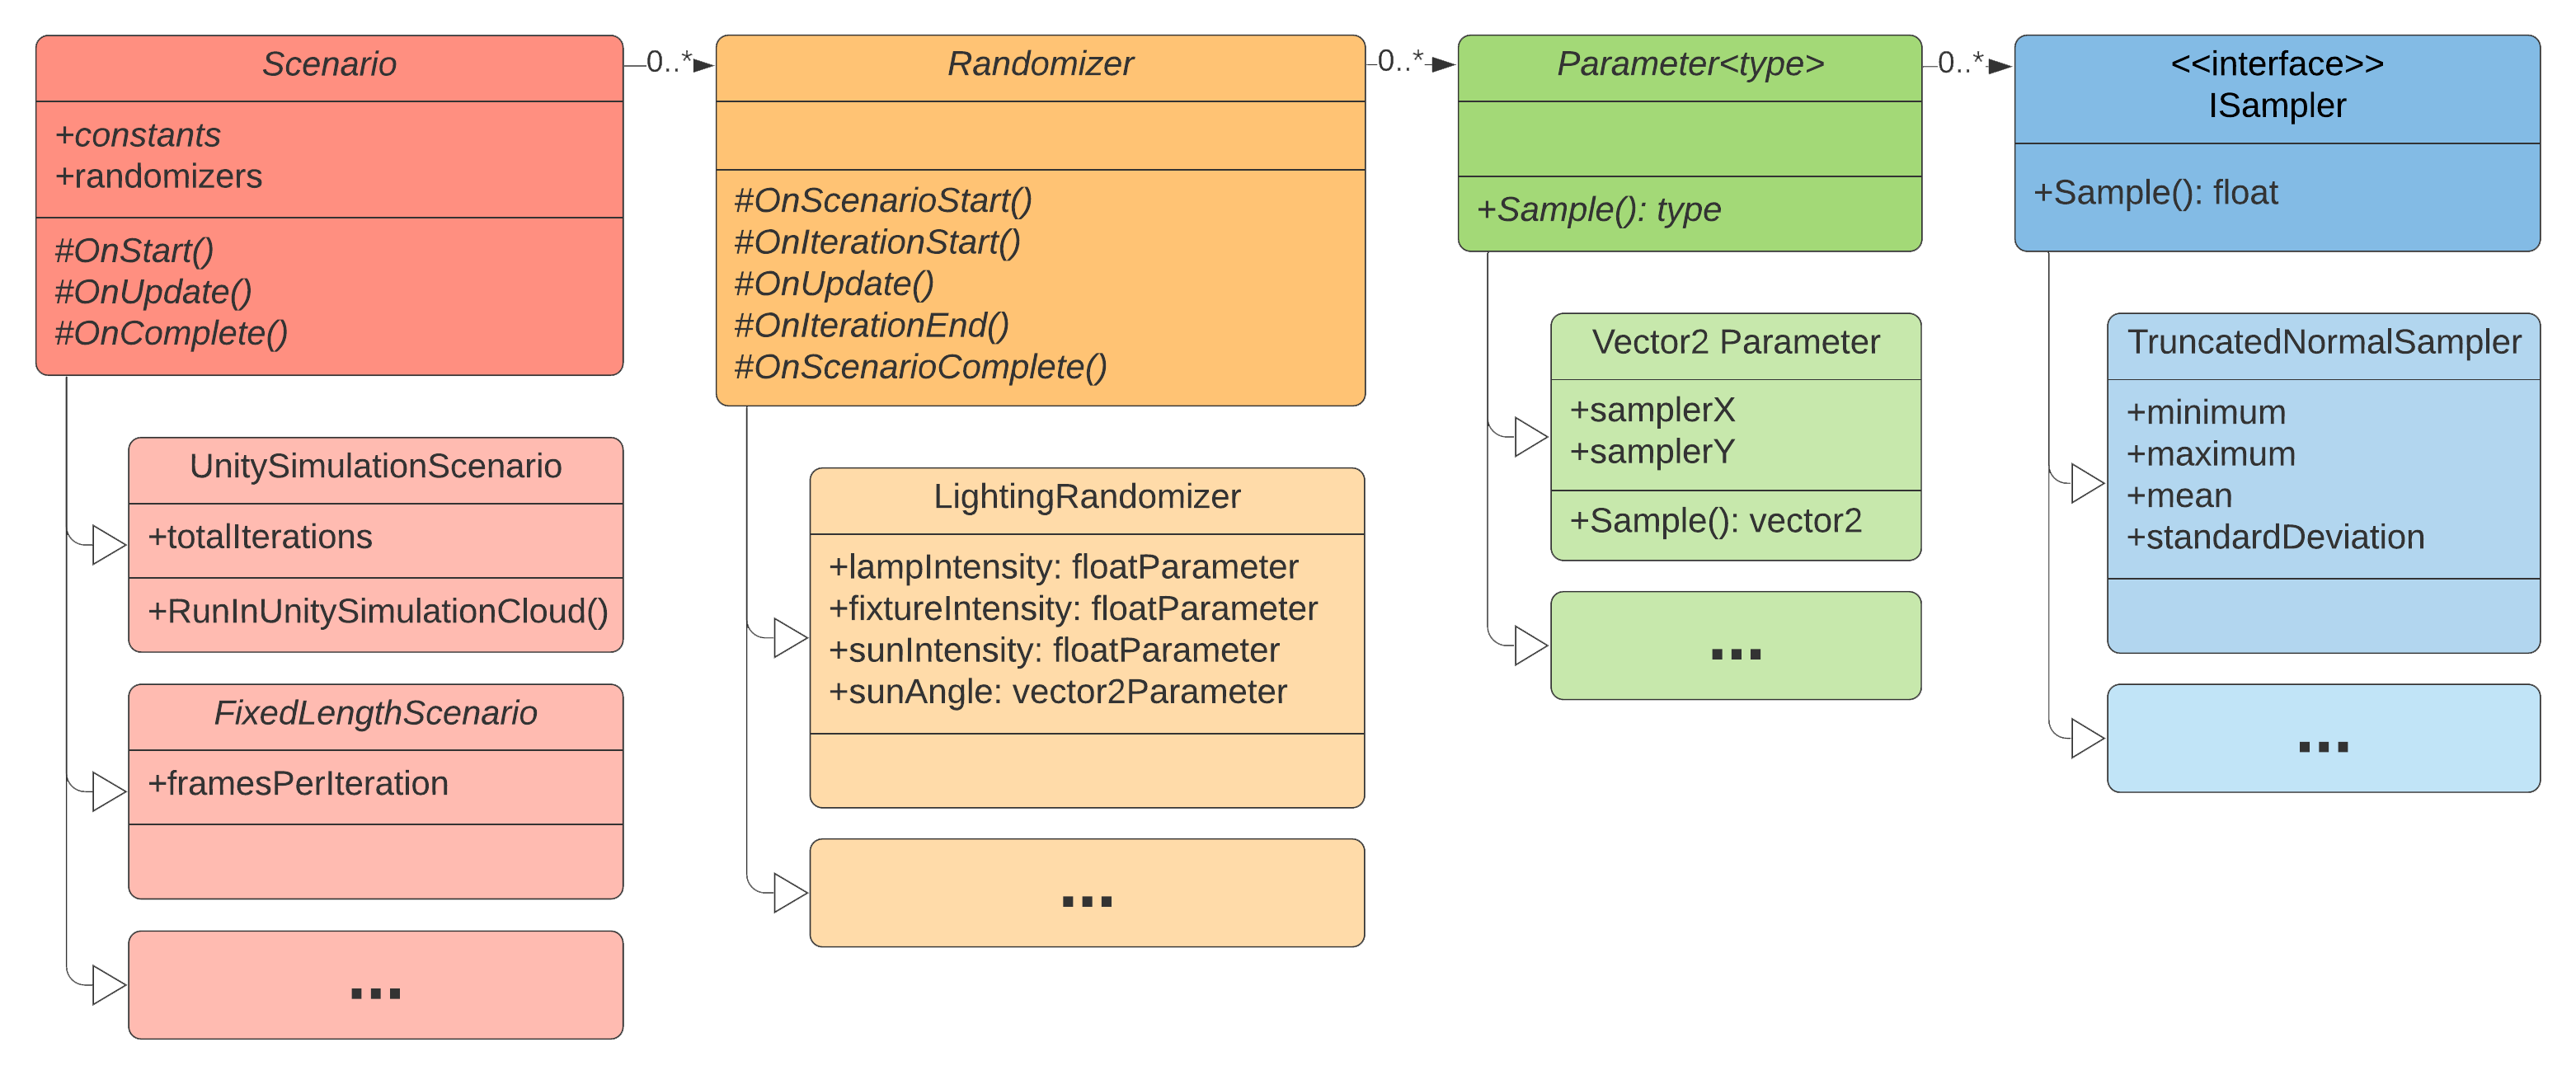
\includegraphics[width=0.99\textwidth]{Figures/randomization_uml.png}
    \caption{UML diagram of the randomization framework in the Unity Perception package, showing the relationships between randomizers, parameters, and interfaces. Taken from Unity Perception package documentation \cite{UMLdiagram}.}
    \label{fig:randomizer class uml}
    
\end{figure}

\subsubsection{RotationRandomizer}
The \textit{RotationRandomizer} \cite{rotation_randomizer} applies a random roll, pitch, and yaw to a 3D object in each iteration. It builds on the \textit{Randomizer} class and takes in six float parameters: the minimum and maximum rotation for the x, y, and z axes. The \texttt{OnIterationStart()} method then runs, which picks a random rotation within the specified ranges. The use of a minimum and maximum is important for this project to ensure the object doesn’t end up upside down or floating in unrealistic positions.

\subsubsection{SunAngleRandomizer}
The second randomizer used is the \textit{SunAngleRandomizer} \cite{sun_angle_randomizer}. This randomizer manipulates the light source connected to the camera to simulate different times of the day. It takes in five parameters: the minimum and maximum for the time of day and the day of the year (where 0 corresponds to January 1st and 356 corresponds to December 31st). The last parameter is the latitude, which is important for calculating the suns position at a given time.

\subsubsection{ColorRandomizer}
The last randomizer used in this project is the \textit{ColorRandomizer} \cite{color_randomizer}. This randomizer allows the randomization of an object's color by adjusting the RGBA (Red, Green, Blue, and Alpha) components within specified ranges. It takes parameters for the minimum and maximum values for each of the components, which generates a color variation to objects. Similar to the other randomizers, the \textit{ColorRandomizer} uses the \texttt{OnIterationStart()} method to apply the randomization on each frame.


\subsection{Customizable Randomizers}
Additional randomizers was coded to make the dataset more varied and random than what the perception package offers by default. These custom randomizers control camera positioning, object placement, and environmental effects. All new scripts are written in C\# and are based on the perception class Randomizer.

\subsubsection{Camera Randomizer}
The \textit{Camera Randomizer} generates a new camera position for each frame while ensuring that the camera remains focused on the target object. By extending the \textit{Randomizer} class, this custom randomizer provides control over the camera's distance from the object, as well as its pitch (elevation) and yaw (horizontal rotation) angles. \\

\noindent Spherical coordinates were used to calculate new camera positions. The randomizer takes user-defined ranges for distance, pitch, and yaw, and calculates a random value within these ranges for each iteration. These parameters are then converted to Cartesian coordinates using the following equations:

\begin{align}
X_{\text{offset}} &= d \cdot \sin(\phi) \cdot \cos(\theta) \\
Y_{\text{offset}} &= d \cdot \sin(\theta) \\
Z_{\text{offset}} &= d \cdot \cos(\phi) \cdot \cos(\theta)
\end{align}

\noindent In the equations is \(d\) the camera's distance from the object, \(\phi\) is the yaw angle (in radians), and \(\theta\) is the pitch angle (in radians). The equations used to convert spherical coordinates to Cartesian coordinates are based on standard mathematical principles \cite{wolfram_spherical_coordinates}.\\

\noindent The calculated offsets determine the new camera position relative to its initial position. The camera is then rotated to face the target object using Unity's \texttt{Quaternion.LookRotation} function to calculate the rotation. This function takes in \texttt{target.position - offset.position}, which gives the relative position of the target from the camera's current position, and calculates the transformation \cite{unity_quaternion_lookrotation}. This randomizer generates varied camera perspectives, capturing different views of the object, the water-level and background elements.

\begin{figure}[H]
    \centering
    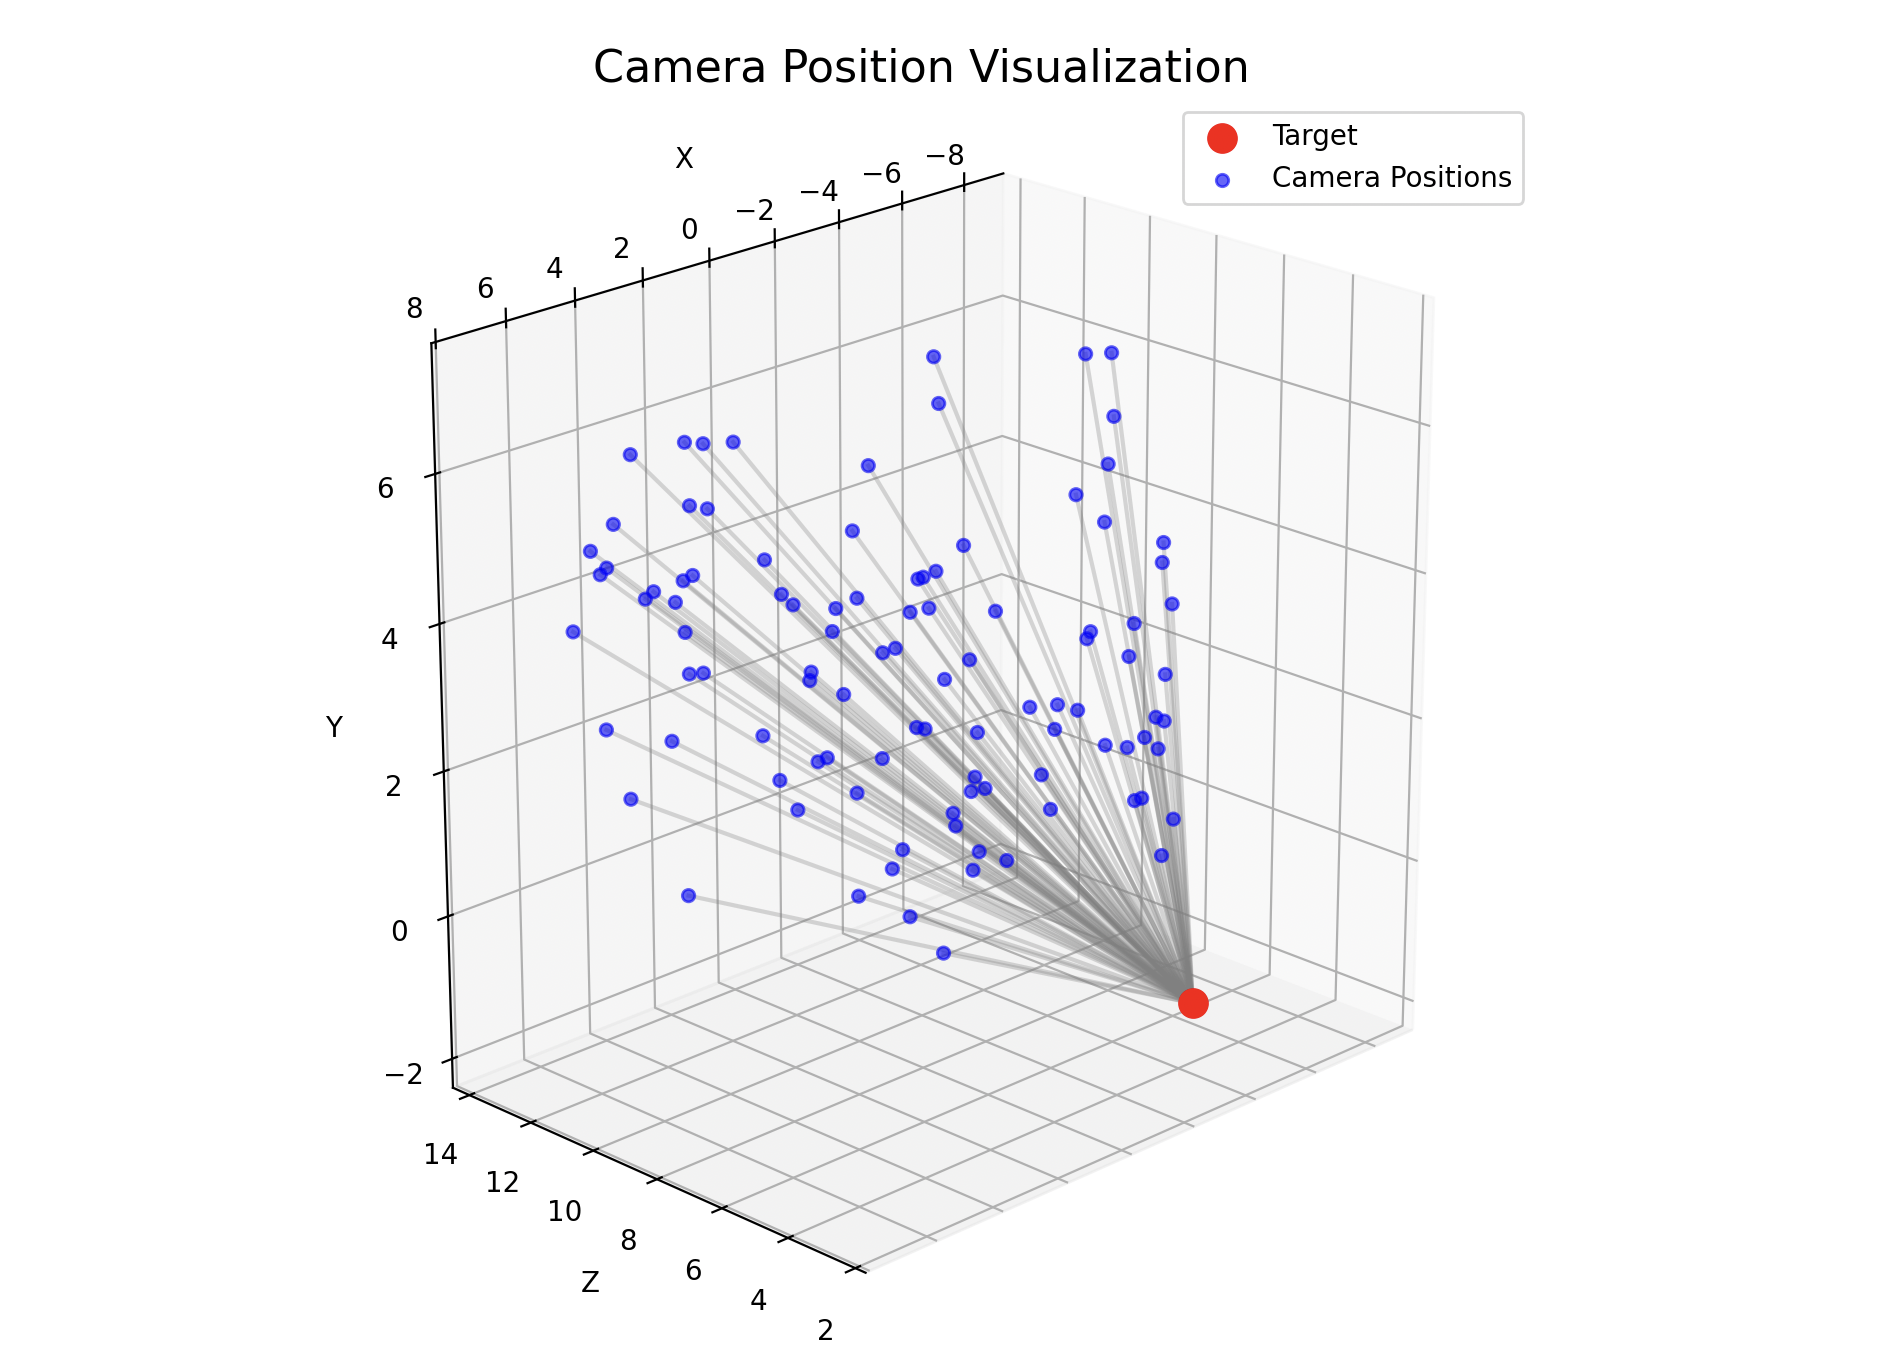
\includegraphics[width=0.7\textwidth]{Figures/camerapos.png}
    \caption{Visualization of new camera positions generated relative to the initial position.}
    \label{fig:camera_randomizer_plot}
    
\end{figure}

\subsubsection{Position Randomizer}
The \textit{Position Randomizer} changes the location of objects within a specified 3D space. It builds on the Randomizer class and allows users to define ranges for the X and Z positions. Random values within these ranges are generated, and the object is moved to a new position while keeping its original Y position unchanged. This ensures the object's height stays the same, as the scene simulate floating objects. This randomizer ensures objects are placed off-center, adding spatial variety.

\subsubsection{Rain Randomizer}
The \textit{Rain Randomizer} enhances the dataset by simulating rain effects during data collection. It includes a parameter that sets how many iterations the rain effect will be applied. After reaching this limit, the rain effect turns off, and the remaining iterations are generated without it. This adds realistic noise and variety to the scene, improving the diversity of the dataset.

